\vspace{10pt}

{\centering\subsection*{张锦:如何引导不爱阅读的孩子阅读?}}

\addcontentsline{toc}{subsection}{张锦:如何引导不爱阅读的孩子阅读?}

\renewcommand{\leftmark}{张锦:如何引导不爱阅读的孩子阅读?}

\begin{figure}[htbp]

\centering

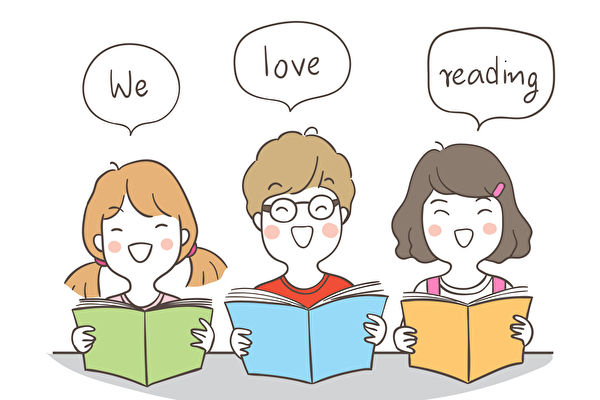
\includegraphics[width = .5\textwidth]{./ch/v2.jpg}

\end{figure}




这一周很高兴看到更多的家长参与到分享中来,并且看到大家非常注重家庭的阅读氛围,这非常的好。感谢才俊、宇州、贤文的分享,也期待更多家长参与到分享中来。






关于张锦:如何引导不爱阅读的孩子阅读,我想分享我的一些想法。



第一,没有孩子不爱阅读,只是没有找到孩子的“兴奋点”。需要尝试不同类型的图书引导孩子去阅读,书的种类有很多。



第二,故事化阅读。孩子不爱阅读?OK。咱们找本适龄的图书,加入家长们自己的口语化叙述,以口语讲故事的形式说给孩子们听,以引导孩子们的好奇心为主。



第三,生活导向阅读。孩子们平时生活中没有各种疑问吗?我想总会有的。OK,机会来了,以孩子们的问题/提问为切入点,找到与孩子们的疑惑相关的图书,指引孩子们自己去看,并引导他们自己找到答案,并结合自己的理解,讲述给我们家长听。



大家怎么看呢?谢谢大家。

\vspace{10pt}

作者:张锦

朗读:张锦

发布:2021年4月17日



\vspace{10pt}

\hline

